\documentclass[a4paper,11pt]{article}

\usepackage[T1]{fontenc}
\usepackage[polish]{babel}
\usepackage[utf8]{inputenc}
\usepackage{lmodern}
\selectlanguage{polish}
\usepackage[top=2cm, bottom=2cm, left=3cm, right=3cm]{geometry}

\makeatletter
\newcommand{\linia}{\rule{\linewidth}{0.4mm}}
\renewcommand{\maketitle}{\begin{titlepage}
    \vspace*{2cm}
    \begin{center}\LARGE
    Politechnika Warszawska\\
    Wydział Elektryczny\\
    \end{center}
    \vspace{5cm}
    \noindent\linia
    \begin{center}
      \LARGE \textsc{\@title}
         \end{center}
     \linia
    \vspace{0.5cm}
    \begin{flushright}
    \begin{minipage}{5cm}
    \textit{Autorzy:}\\
    \normalsize \textsc{\@author} \par
    \end{minipage}
    \vspace{5cm}
     \end{flushright}
    \vspace*{\stretch{6}}
    \begin{center}
    \@date
    \end{center}
  \end{titlepage}%
}
\makeatother
\author{Grzegorz Kopyt\\
Daniel Sporysz}
\title{Specyfikacja Implementacyjna \\
"WireWorld"}

\usepackage{graphicx}
\begin{document}

\maketitle


\tableofcontents
\vspace{1cm}
\noindent\linia





\section{Diagram klas}


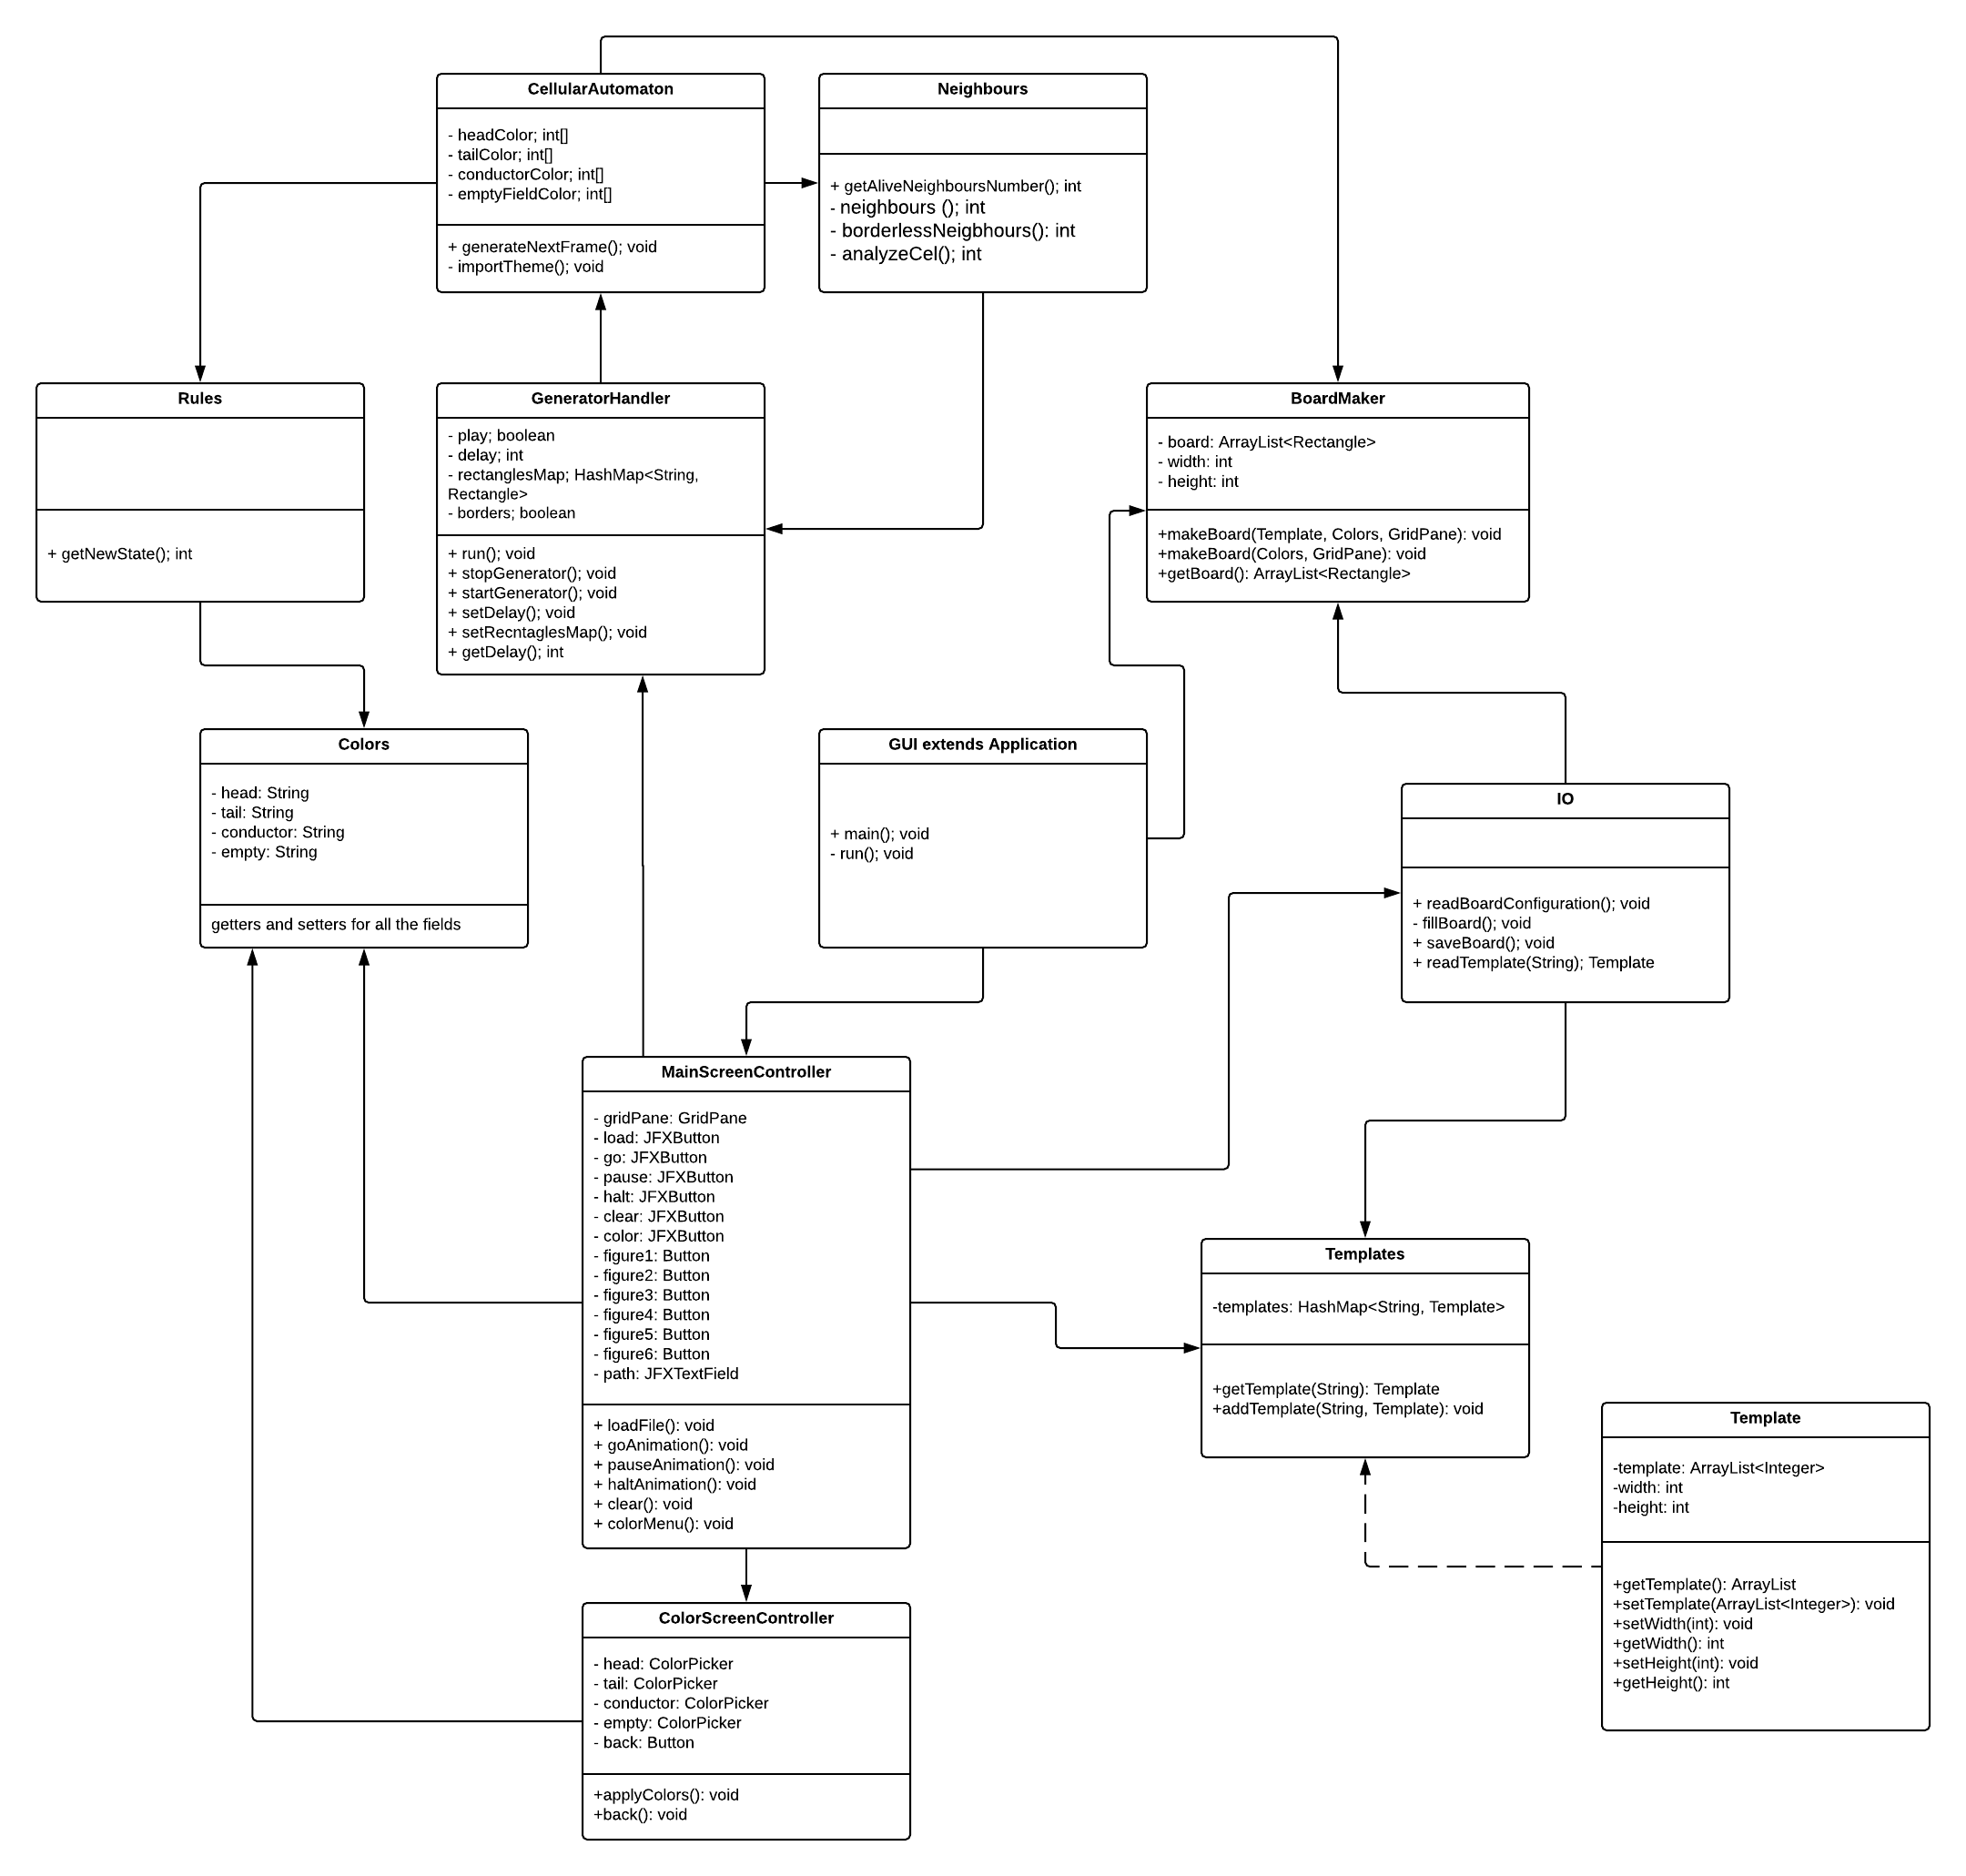
\includegraphics[width=\textwidth]{DiagramKlas}

\noindent\linia


\section{Diagram pakietów}
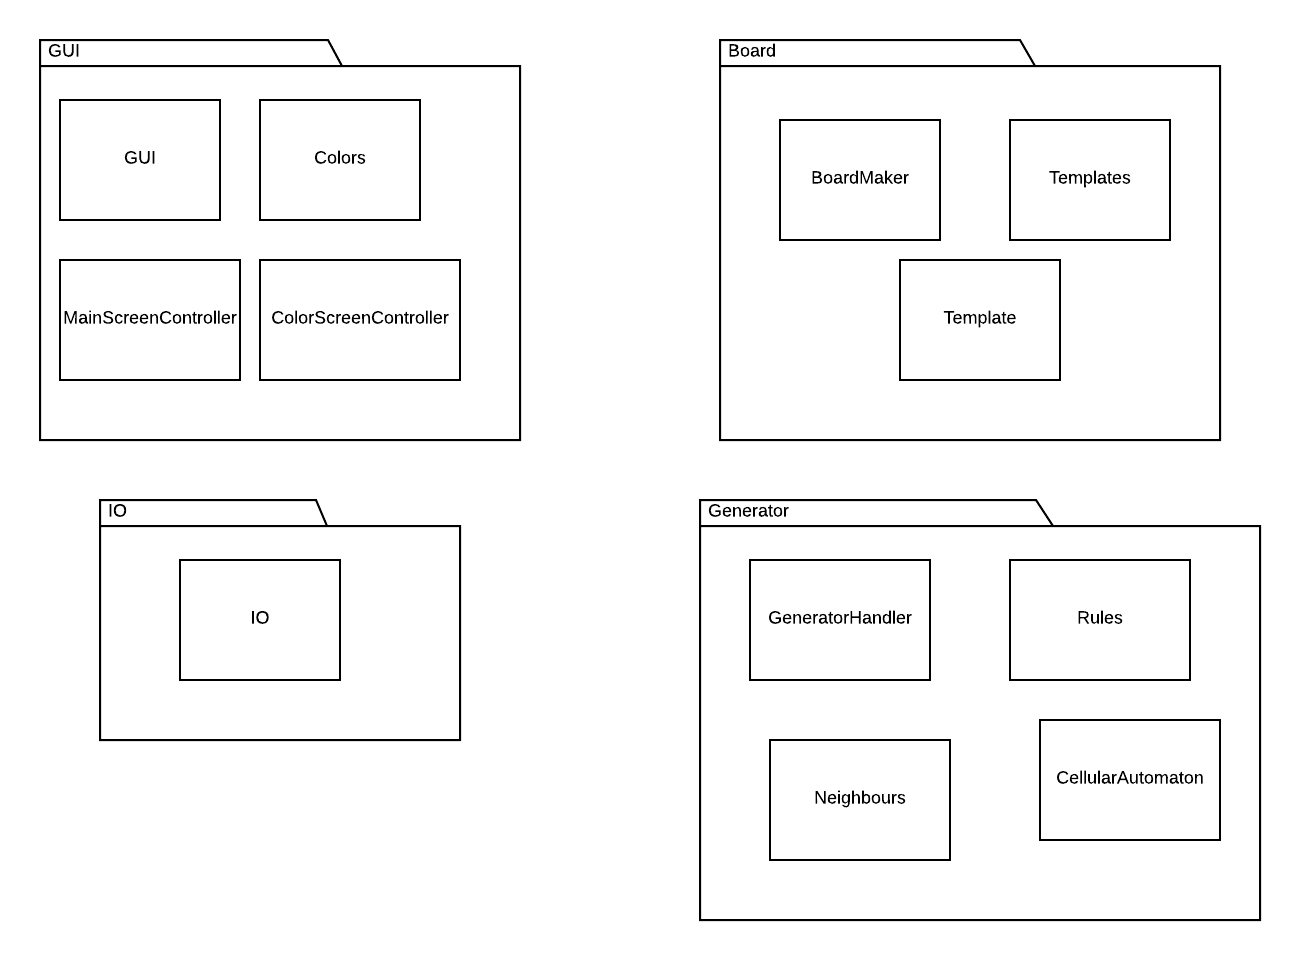
\includegraphics[width=\textwidth]{DiagramPakiet}







\noindent\linia
\section{Pakiet GUI}

Zawiera dodatkową bibliotekę: jfoenix.

\subsection{Pliki .fxml:}
\begin{itemize}
\item MainScreen.fxml
\item ColorScreen.fxml
\end{itemize}
\noindent\linia

\subsection{GUI}
Rozszerza klasę Application z javafx.
\subsubsection{Pola}
brak
\subsubsection{Metody}
\begin{itemize}
\item \textbf{main}

Standardowo wywołuje metodę launch.
\item \textbf{start}

Wczytuje plik MainScreen.fxml, przygotowuje całą scenę i wyświetla ją w wymiarach (800, 600).
\end{itemize}


\subsection{MainScreenController}
Kontroler sceny MainScreen.fxml.
\subsubsection{Pola}
\begin{itemize}
\item GridPane gridPane
\item JFXButton load
\item JFXButton go
\item JFXButton pause
\item JFXButton halt
\item JFXButton clear
\item JFXButton color
\item Button figure1
\item Button figure2
\item Button figure3
\item Button figure4
\item Button figure5
\item Button figure6
\item JFXTextField path
\end{itemize}
\subsubsection{Metody}
\begin{itemize}
\item \textbf{loadFile}

Standardowo wywołuje metodę launch.
\item \textbf{goAnimation}

Uruchamia animacje wywołując metodę z klasy Animation.
\item \textbf{pauseAnimation}

Pauzeuje animacje metodą z klasy Animation.
\item \textbf{haltAnimation}

Powoduje powrót animacji do punktu początkowego.
\item \textbf{clear}

Zmienia kolor każdej komórki w tablicy na biały.
\item \textbf{colorMenu}

Wyświetla okno z pliku ColorMenu.fxml
\end{itemize}





\subsection{ColorScreenController}
Kontroler sceny ColorScreen.fxml.
\subsubsection{Pola}
\begin{itemize}
\item ColorPicker head
\item ColorPicker tail
\item ColorPicker conductor
\item ColorPicker empty

\end{itemize}
\subsubsection{Metody}
\begin{itemize}
\item \textbf{back}

Powoduje powrót do MainScreen.
\item \textbf{applyColors}

Pobiera z obiektów klasy ColorPicker informacje o kolorach i przekazuje je klasie Colors.

\end{itemize}
\noindent\linia




\subsection{Colors}
Kontroler sceny ColorScreen.fxml.
\subsubsection{Pola}
\begin{itemize}
\item String head
\item String tail
\item String conductor
\item String empty

\end{itemize}
\subsubsection{Metody}
\begin{itemize}
\item \textbf{getHead}
\item \textbf{setHead}
\item \textbf{getTail}
\item \textbf{setTail}
\item \textbf{getConductor}
\item \textbf{setConductor}
\item \textbf{getEmpty}
\item \textbf{setEmpty}

\end{itemize}
\noindent\linia







\section{Pakiet IO}
\subsection{IO}
krótki opis klasy
\subsubsection{Pola}

\subsubsection{Metody}



\noindent\linia

\section{Pakiet Board}

\subsection{BoardMaker}
Odpowiada za stworzenie tablicy obiektów klasy Rectangle. Tablica ta będzie służyła jako obszar edytowany przez użytkownika, a także będzie na niej wyświetlana animacja.
\subsubsection{Pola}

\subsubsection{Metody}




\subsection{Factory}
krótki opis klasy
\subsubsection{Pola}

\subsubsection{Metody}

\noindent\linia

\section{Pakiet Generation}

\subsection{Animation}
krótki opis klasy
\subsubsection{Pola}

\subsubsection{Metody}

\noindent\linia
\section{Przepływ Sterowania}




\noindent\linia
\section{Testy klas i pakietów}


\subsection{GUI}
\begin{description}

\item[Scenariusze] \hfill
\begin{enumerate}
\item
\item 
\item
\item
\item 
\end{enumerate}

\item[Kryteria oceny poprawnej pracy] \hfill
\begin{enumerate}
\item 
\item
\item
\item 
\item 
\end{enumerate}

\end{description}


\end{document}



